\documentclass[aspectratio=169]{beamer}
\usepackage{will_handley}
\newcommand{\av}[2][]{\left\langle #2\right\rangle_{#1}}

% Commands
% --------
% - \arxiv{arxiv number}
% - \cols{width}{lh column}{rh column}
% -  \begin{fig(left|right)}[fractional width (e.g 0.6) ]{name of image}
%        content of other column
%    \end{fig(left|right)}

% Talk details
% ------------
\title{Frontiers of Nested Sampling}
\date{20\textsuperscript{th} July 2022}
%Nested Sampling is an established numerical technique for optimising,
%sampling, integrating and scanning *a priori* unknown probability
%distributions. Whilst typically used in the context of traditional
%likelihood-driven Bayesian inference, it's capacity as a general sampler means
%that it is capable of exploring distributions on data [2105.13923] and joint
%spaces [1606.03757].  
%
%In this talk I will give a brief outline of the points
%of difference of nested sampling in comparison with other techniques, what it
%can uniquely offer in tackling the challenge of likelihood-free inference, and
%discuss ongoing work with collaborators in applying it in a variety of
%LFI-based approaches.

\begin{document}

\begin{frame}
    \titlepage
\end{frame}

\begin{frame}
    \frametitle{Highlight: state-of-the-art Nature review}
    \begin{columns}
        \column{0.5\textwidth}
        \begin{itemize}
            \item Invented by John Skilling in 2004.
            \item Recent Nature review primer on nested sampling led by Andrew Fowlie and assembled by the community.
            \item Showcases the current set of tools, and applications from chemistry to cosmology.
            \item In this talk
                \begin{itemize}
                    \item Reminder on theory of nested sampling,
                    \item Updates to the meta algorithm since 2004,
                    \item Updates to the set of tools surrounding nested sampling,
                    \item Future research projects.
                \end{itemize}
        \end{itemize}
        \column{0.3\textwidth}
        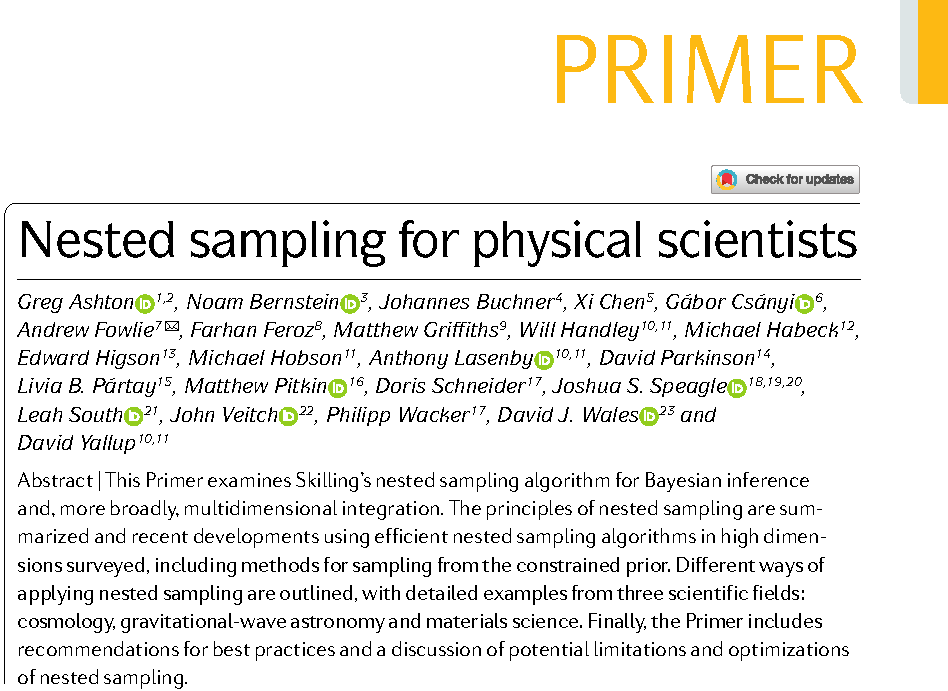
\includegraphics[width=\textwidth]{figures/nature1}
        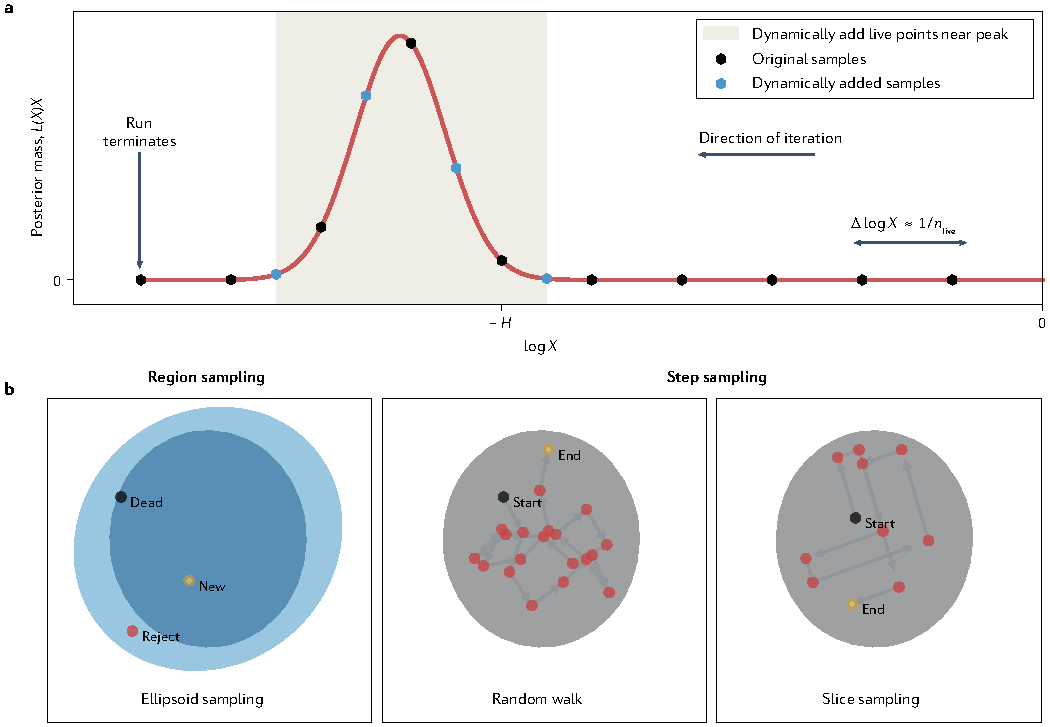
\includegraphics[width=\textwidth]{figures/nature2}
        \column{0.2\textwidth}
        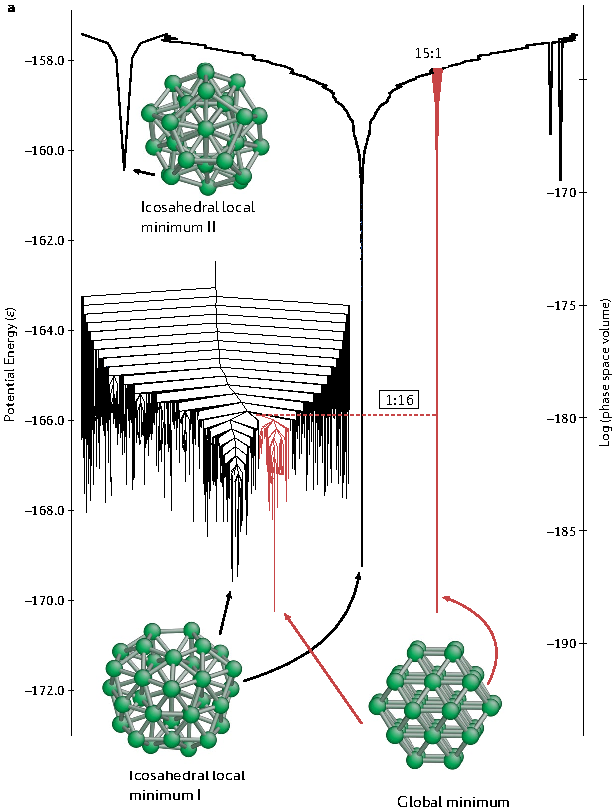
\includegraphics[width=\textwidth]{figures/nature4}
        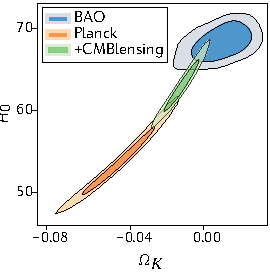
\includegraphics[width=\textwidth]{figures/nature5}
    \end{columns}

\end{frame}

\begin{frame}
    \frametitle{What is Nested Sampling?}
    \begin{itemize}
        \item Nested sampling is a multi-purpose numerical mathematical tool.
        \item Given a (scalar) function $f$ with a vector of parameters $\theta$, it can be used for:
    \end{itemize}
    \vspace{-10pt}
    \begin{columns}[t]
        \column{0.33\textwidth}
        \begin{block}{Optimisation}
            \vspace{-5pt}
            \[\theta_\mathrm{max} = \max_\theta{f(\theta)}\]
        \end{block}
        \column{0.33\textwidth}
        \begin{block}{Sampling}
            \vspace{-5pt}
            \[\text{draw }\theta\sim f\]
        \end{block}
        \column{0.33\textwidth}
        \begin{block}{Integration}
            \vspace{-5pt}
            \[\int f(\theta) dV \]
            \vspace{-15pt}
        \end{block}
    \end{columns}
    \begin{columns}[t]
        \column{0.33\textwidth}
        \centerline{\includegraphics[width=0.8\textwidth,page=13]{figures/himmelblau}}
        \column{0.33\textwidth}
        \centerline{\includegraphics[width=0.8\textwidth,page=15]{figures/himmelblau}}
        \column{0.33\textwidth}
        \centerline{\includegraphics[width=0.8\textwidth,page=14]{figures/himmelblau}}
    \end{columns}
\end{frame}

\begin{frame}
    \frametitle{MCMC sampling}
    \begin{columns}
        \column{0.6\textwidth}
        \begin{itemize}
            \item Markov chain based methods generate samples from posterior distribution by a stepping procedure.
            \item This can get stuck in local peaks.
            \item Cannot compute normalisation $\mathcal{Z}$ of Bayes theorem:
                \[ \C[0]{P(\theta|D,M)} = \frac{\C[2]{P(D|\theta,M)}\C[1]{P(\theta|M)}}{\C[3]{P(D|M)}},\]
                \[ \C[0]{\mathcal{P}} = \frac{\C[2]{\mathcal{L}}\times \C[1]{\pi}}{\C[3]{\mathcal{Z}}}, \qquad \C[0]{\text{posterior}} = \frac{\C[2]{\text{likelihood}}\times \C[1]{\text{prior}}}{\C[3]{\text{evidence}}}. \]
            \item We generally want the evidence $\C[3]{\mathcal{Z}=P(D|M)}$ for the second stage of inference: model comparison:
                \[ P(M|D) = \frac{\C[3]{P(D|M)}P(M)}{P(D)}, \qquad \text{Science}(M) = \frac{\C[3]{\mathcal{Z}_M} \Pi_M}{\sum_m \C[3]{\mathcal{Z}}_m \Pi_m}. \]

        \end{itemize}
        \column{0.4\textwidth}

        \includegraphics<1>[width=\textwidth,page=16]{figures/himmelblau}%
        \includegraphics<2>[width=\textwidth,page=17]{figures/himmelblau}%
        \includegraphics<3>[width=\textwidth,page=18]{figures/himmelblau}%
        \includegraphics<4>[width=\textwidth,page=19]{figures/himmelblau}%
        \includegraphics<5>[width=\textwidth,page=20]{figures/himmelblau}%
        \includegraphics<6>[width=\textwidth,page=21]{figures/himmelblau}%

    \end{columns}
\end{frame}

\begin{frame}
    \frametitle{Nested sampling}
    \begin{columns}
        \column{0.6\textwidth}
        \begin{itemize}
            \item Nested sampling: completely different way to sample.
            \item Ensemble sampling to compress prior to posterior.
            \item Sequentially update a set $S$ of $n$ samples:
                \begin{itemize}
                    \item[$S_0$:]  Generate $n$ samples uniformly over the space (from the prior $\pi$). 

                    \item[$S_{i+1}$:] Delete the lowest likelihood sample in $S_{i}$, and replace it with a new uniform sample with higher likelihood.
                \end{itemize}
            \item Requires one to be able to sample uniformly within a region, subject to a {\em hard likelihood constraint}:
                \[\{\theta\sim \pi : \mathcal{L}(\theta)>\mathcal{L}_*. \}\]
            \item This procedure optimises (multimodally), and can calculate the \C[3]{evidence} \& \C[0]{posterior} weights.
        \end{itemize}
        \column{0.4\textwidth}

        \includegraphics<1|handout:0>[width=\textwidth,page=1]{figures/himmelblau}%
        \includegraphics<2|handout:0>[width=\textwidth,page=2]{figures/himmelblau}%
        \includegraphics<3|handout:0>[width=\textwidth,page=3]{figures/himmelblau}%
        \includegraphics<4          >[width=\textwidth,page=4]{figures/himmelblau}%
        \includegraphics<5|handout:0>[width=\textwidth,page=5]{figures/himmelblau}%
        \includegraphics<6|handout:0>[width=\textwidth,page=6]{figures/himmelblau}%
        \includegraphics<7|handout:0>[width=\textwidth,page=7]{figures/himmelblau}%
        \includegraphics<8|handout:0>[width=\textwidth,page=8]{figures/himmelblau}%

    \end{columns}
\end{frame}

\begin{frame}
    \frametitle{Mathematics of Nested Sampling}
    \framesubtitle{A probabilistic Lebesgque integrator}
    \begin{columns}
        \column{0.5\textwidth}
        \begin{itemize}
            \item At each iteration, the likelihood contour will shrink in volume by  $\approx 1/n$.
            \item Nested sampling zooms in to the peak of the function $\mathcal{L}$ {\em exponentially}.
                \vspace{-5pt}
                \[
                    \mathcal{Z} \approx \sum_i \Delta\mathcal{L}_i X_{i}, \quad
                    X_{i+1} \approx \frac{n}{n+1}X_i, \quad X_{0} = 1 .
                \]
                \vspace{-15pt}
            \item Although this is only approximate, we can quantify the error 
                \vspace{-10pt}
                \[
                    P(X_i|X_{i-1}) = \frac{X_{i}^{n-1}}{nX_{i-1}^n}\times[0<X_i<X_{i-1}].
                \]
                \vspace{-15pt}
            \item Integral can be discretised in several ways
                \vspace{-10pt}
                \[
                    \mathcal{Z} \approx \sum_i \Delta\mathcal{L}_i X_{i} = \sum_i \mathcal{L}_i \Delta X_{i} = \sum_i \tfrac{\mathcal{L}_i+\mathcal{L}_{i-1}}{2}{\small(X_{i-1}-X_i).}
                \]

        \end{itemize}
        \column{0.5\textwidth}
        \includegraphics<1|handout:0>[width=\textwidth,page=1]{figures/lesbesgue}%
        \includegraphics<2|handout:0>[width=\textwidth,page=2]{figures/lesbesgue}%
        \includegraphics<3|handout:0>[width=\textwidth,page=3]{figures/lesbesgue}%
        \includegraphics<4|handout:0>[width=\textwidth,page=4]{figures/lesbesgue}%
        \includegraphics<5|handout:0>[width=\textwidth,page=5]{figures/lesbesgue}%
        \includegraphics<6|handout:0>[width=\textwidth,page=6]{figures/lesbesgue}%
        \includegraphics<7|handout:0>[width=\textwidth,page=7]{figures/lesbesgue}%
        \includegraphics<8|handout:0>[width=\textwidth,page=8]{figures/lesbesgue}%
        \includegraphics<9|handout:0>[width=\textwidth,page=9]{figures/lesbesgue}%
        \includegraphics<10|handout:0>[width=\textwidth,page=10]{figures/lesbesgue}%
        \includegraphics<11|handout:0>[width=\textwidth,page=11]{figures/lesbesgue}%
        \includegraphics<12|handout:0>[width=\textwidth,page=12]{figures/lesbesgue}%
        \includegraphics<13|handout:0>[width=\textwidth,page=13]{figures/lesbesgue}%
        \includegraphics<14|handout:0>[width=\textwidth,page=14]{figures/lesbesgue}%
        \includegraphics<15|handout:0>[width=\textwidth,page=15]{figures/lesbesgue}%
        \includegraphics<16          >[width=\textwidth,page=16]{figures/lesbesgue}%
    \end{columns}
\end{frame}

\begin{frame}
    \frametitle{Dead points: posteriors \& evidences}
    \begin{columns}
        \column{0.6\textwidth}
        \begin{itemize}
            \item At the end, one is left with a set of discarded points.
            \item These may be weighted to form weighted posterior samples using $w_i = \mathcal{L}_i \Delta X_i$.
            \item They can also be used to calculate the normalisation $\mathcal{Z} = \sum \mathcal{L}_i \Delta X_i$, or more generally $\sum_i f(\mathcal{L}_i) \Delta X_i$.
                \begin{itemize}
                    \item Nested sampling probabilistically estimates the volume of the parameter space
                        \[X_i \approx {\left(\frac{n}{n+1}\right)} X_{i-1} \quad\Rightarrow\quad
                        X_i \approx {\left(\frac{n}{n+1}\right)}^i \approx e^{-i/n}, \]
                    \item Nested sampling thus estimates the density of states,
                    \item it is therefore a partition function calculator
                        $Z(\beta) = \sum_i \mathcal{L}_i^\beta \Delta X_i$.
                \end{itemize}
            \item The evolving ensemble of live points allows algorithms to perform self-tuning and mode clustering.
        \end{itemize}

        \column{0.4\textwidth}

        \includegraphics<1|handout:0>[width=\textwidth,page=14]{figures/himmelblau}%
        \includegraphics<2          >[width=\textwidth,page=15]{figures/himmelblau}%

    \end{columns}

\end{frame}

\begin{frame}
  \frametitle{Sampling from a hard likelihood constraint} 
  
  \begin{quote}
    ``It is not the purpose of this introductory paper to develop the technology of navigation within such a volume. We merely note that exploring a hard-edged likelihood-constrained domain should prove to be neither more nor less demanding than exploring a likelihood-weighted space.''
    
   {\hfill --- John Skilling}
  \end{quote}

  \begin{itemize}
      
    \item A large fraction of the work in NS to date has been in attempting to implement a hard-edged sampler in the NS meta-algorithm $\{\theta\sim \pi : \mathcal{L}(\theta)>\mathcal{L}_* \}$.
    \item \url{https://projecteuclid.org/euclid.ba/1340370944}.
    \item There has also been much work beyond this (focus of this talk).
  \end{itemize}
 
\end{frame}


\begin{frame}
    \frametitle{Implementations of Nested Sampling}
    %\begin{columns}
    %    \begin{column}{0.33}
    %        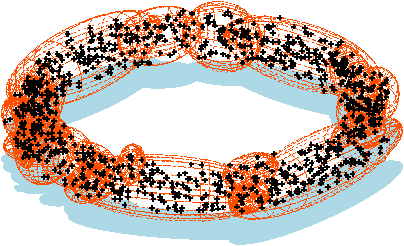
\includegraphics[width=\textwidth]{figures/multinest}
    %    \end{column} 
    %\end{columns}
    \begin{columns}[t]
        \column{0.3\textwidth}
        \texttt{MultiNest}~\arxiv{0809.3437}
        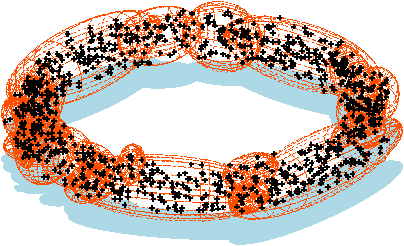
\includegraphics[width=\textwidth]{figures/multinest}
        \texttt{UltraNest}~\arxiv{2101.09604}
        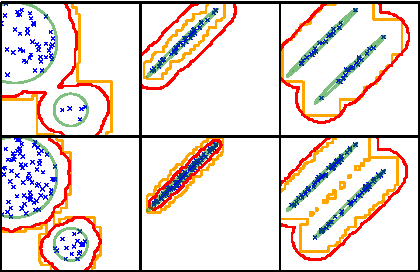
\includegraphics[width=\textwidth]{figures/radfriends}
        \column{0.4\textwidth}
        \texttt{PolyChord}~\arxiv{1506.00171}
        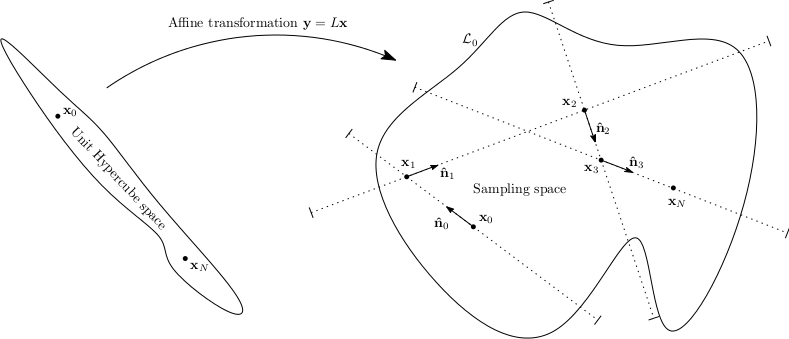
\includegraphics[width=\textwidth]{figures/polychord}
        \vfill
        \texttt{NeuralNest}~\arxiv{1903.10860}
        \begin{columns}
            \column{0.5\textwidth}
            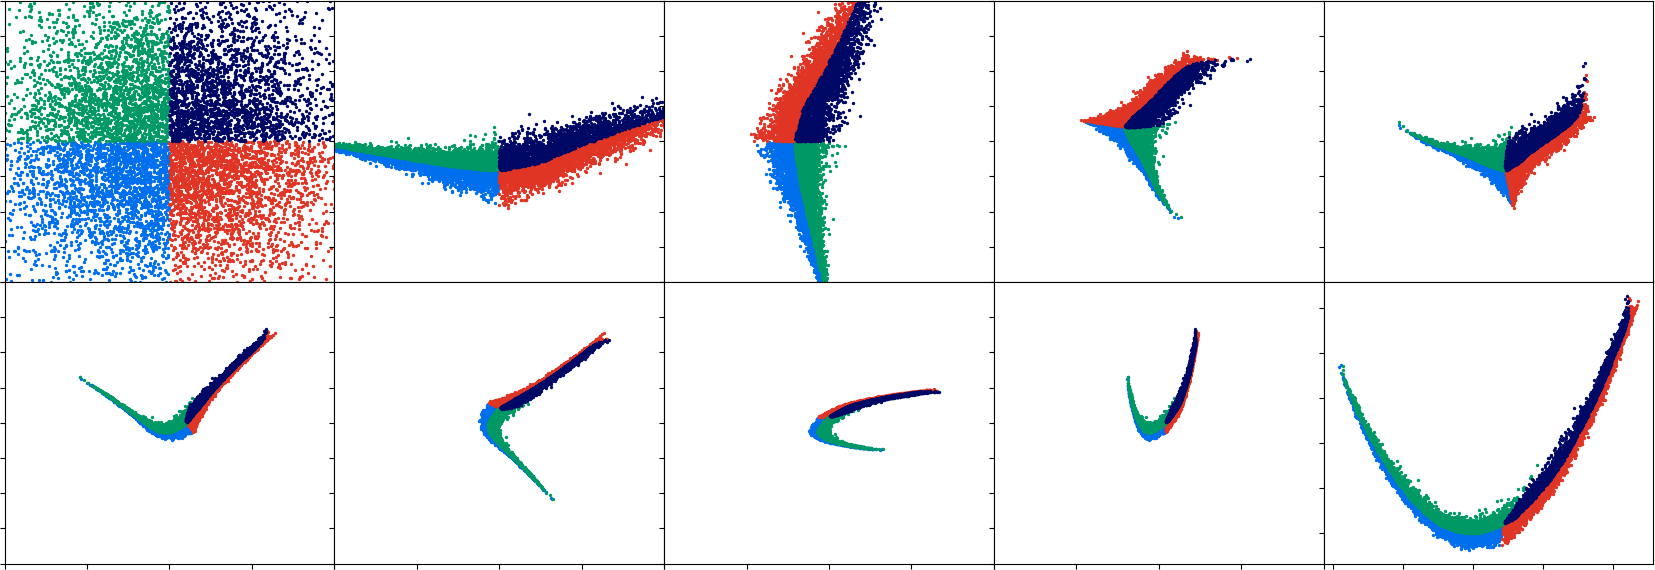
\includegraphics[width=\textwidth]{figures/rosenbrock_flow.png}
            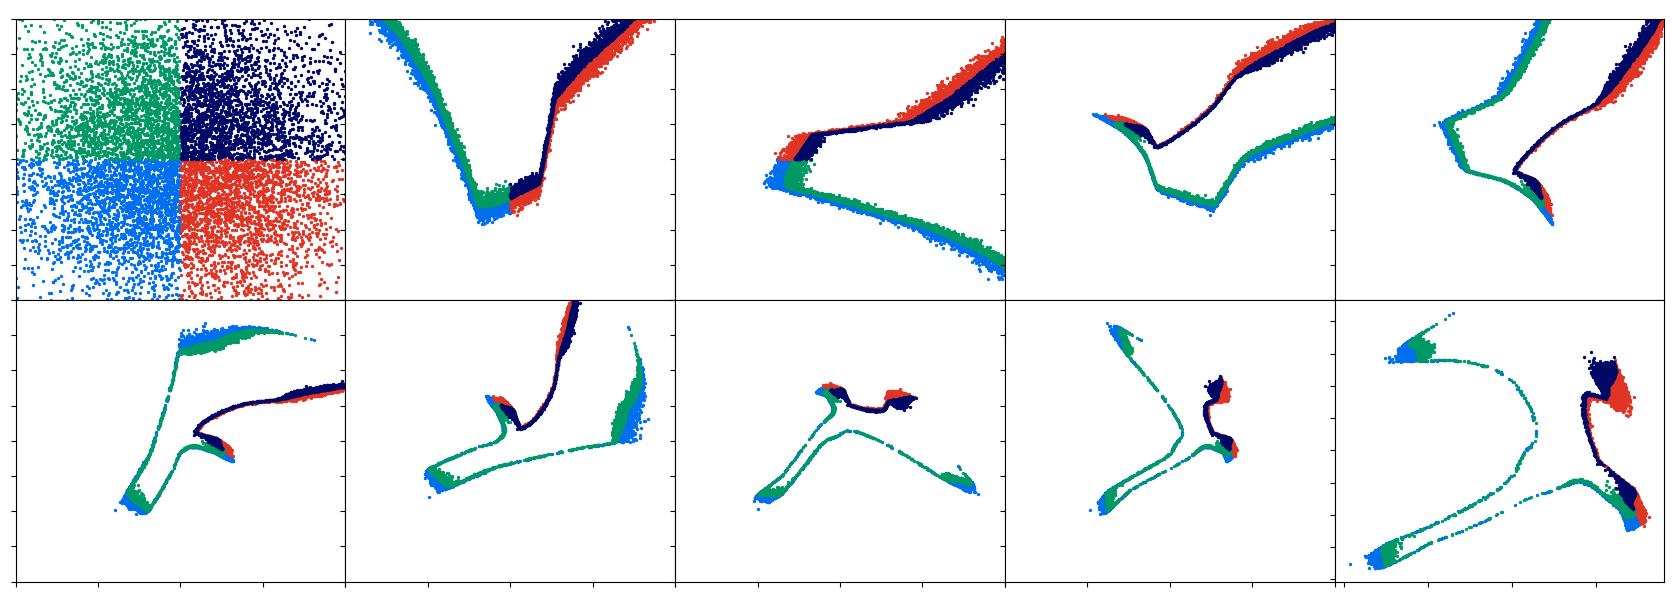
\includegraphics[width=\textwidth]{figures/himmelblau_flow.png}
            \column{0.5\textwidth}
            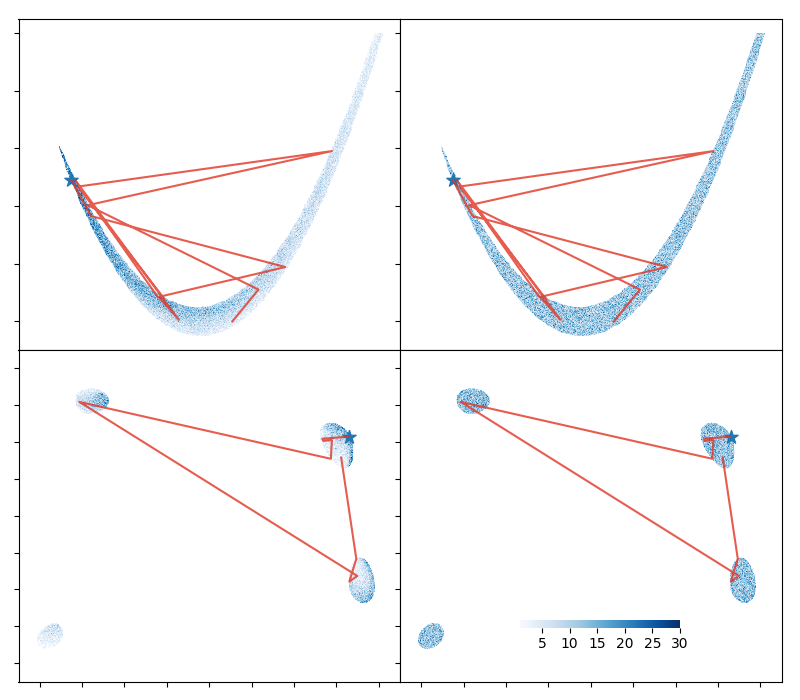
\includegraphics[width=\textwidth]{figures/chains.png}
        \end{columns}
        \texttt{dynesty}~\arxiv{1904.02180}
        \vfill
        \column{0.3\textwidth}
        \texttt{DNest}~\arxiv{1606.03757}
        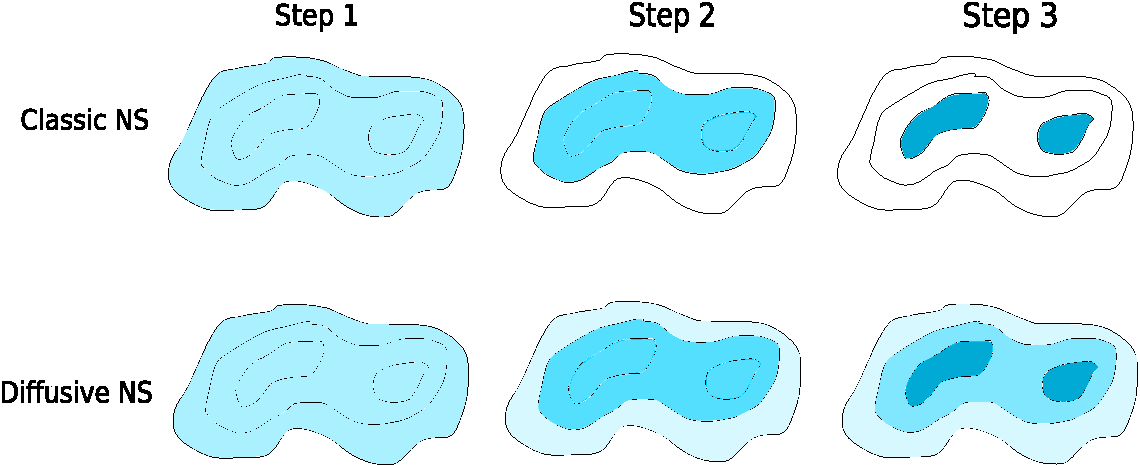
\includegraphics[width=\textwidth]{figures/dnest}
        \texttt{ProxNest}~\arxiv{2106.03646}
        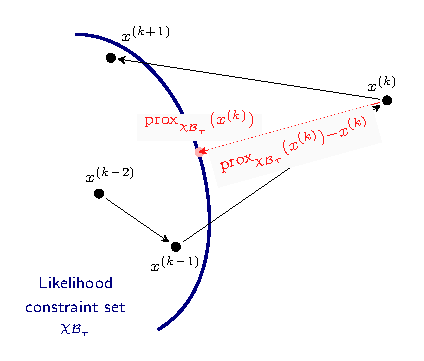
\includegraphics[width=\textwidth]{figures/proxnest_diagram}
        \vfill
    \end{columns}
\end{frame}



\begin{frame}
    \frametitle{Types of nested sampler}
    \begin{itemize}
        \item Broadly, most nested samplers can be split into how they create new live points.
        \item i.e. how they sample from the hard likelihood constraint $\{\theta\sim \pi : \mathcal{L}(\theta)>\mathcal{L}_* \}$.
    \end{itemize}
    \vspace{-10pt}
    \begin{columns}[t]
        \column{0.5\textwidth}
        \begin{block}{Rejection samplers}
            \begin{itemize}
                \item e.g. \texttt{MultiNest}, \texttt{UltraNest}.
                \item Constructs bounding region and draws many invalid points until one is found within $L_*$.
                \item Efficient in low dimensions, exponentially inefficient $\sim\mathcal{O}(e^{d/d_0})$ in high  $d>d_0\sim10$.
            \end{itemize}
        \end{block}
        \column{0.5\textwidth}
        \begin{block}{Chain-based samplers}
            \begin{itemize}
                \item e.g. \texttt{PolyChord}, \texttt{ProxNest}.
                \item Run Markov chain starting at a live point, generating many valid (correlated) points.
                \item Linear $\sim\mathcal{O}(d)$ penalty in decorrelating new live point from the original seed point.
            \end{itemize}
        \end{block}
    \end{columns}
    \vspace{15pt}
    \begin{itemize}
        \item Nested samplers usually come with:
            \begin{itemize}
                \item \emph{resolution} parameter $n_\mathrm{live}$ (which improve results as $\sim\mathcal{O}(n_\mathrm{live}^{-1/2})$.
                    \item set of \emph{reliability} parameters~\arxiv{2101.04525}, which don't improve results if set arbitrarily high, but introduce systematic errors if set too low.
                    \item e.g. \texttt{Multinest} efficiency \texttt{eff} or \texttt{PolyChord} chain length $n_\mathrm{repeats}$.
            \end{itemize}
    \end{itemize}
\end{frame}

\begin{frame}
    \frametitle{Dynamic nested sampling}
    \begin{columns}
        \column{0.3\textwidth}
        \begin{itemize}
            \item Small change to meta-algorithm: 
            \item Allow the number of live points to vary at run time \arxiv{1704.03459}.
        \end{itemize}
        \column{0.7\textwidth}
        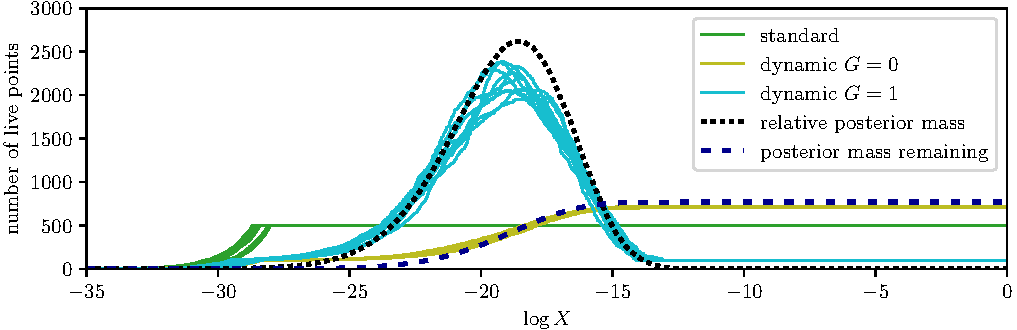
\includegraphics[width=\textwidth]{figures/dynesty}
    \end{columns}
    \begin{columns}
        \column{0.5\textwidth}
        \begin{itemize}
            \item Separate creation and deletion:
                \begin{itemize}
                    \item[$S_0$:] Generate $n$ samples uniformly over the space (from the prior $\pi$). 

                    \item[$S_{i+1}$:] 
                        \begin{itemize}
                            \item Delete the lowest likelihood sample in $S_{i}$ with criterion $D_i$,
                            \item Create  a new uniform sample with higher likelihood with criterion $C_i$.
                        \end{itemize}
                \end{itemize}
            \item Extremely straightforward to implement \\ (just let number of live points $n_i$ vary with $i$).
        \end{itemize}
        \column{0.5\textwidth}
        \begin{itemize}
            \item Need to specify creation and deletion criteria.
            \item This can prove useful, e.g.
                \begin{itemize}
                    \item Killing off all remaining live points is equivalent to usual correction term,
                    \item Oversampling the prior by \texttt{nprior}.
                \end{itemize}
            \item However, DNS is exactly the right level of complexity to get the uninitiated excited, and does not result in dramatic speedups.
        \end{itemize}
    \end{columns}
\end{frame}

\begin{frame}
    \frametitle{Nested sampling post-processing: Weaving and unweaving runs}
    \begin{columns}
        \column{0.7\textwidth}
        \begin{itemize}
            \item There is now a substantial literature on what you can do with a nested sampling run.
            \item John Skilling originally noted that two nested sampling runs can be ``merged'':
                \begin{itemize}
                    \item Take two nested sampling runs on likelihood $\mathcal{L}$ with $n$ live points and $m$ live points each,
                    \item Concatenate the dead points, and re-sort on likelihood,
                    \item The resulting set of points are dead points from an $n+m$-live point run.
                \end{itemize}
            \item To generalise to dynamic nested sampling one needs to record more information.
        \end{itemize}
        \column{0.3\textwidth}
        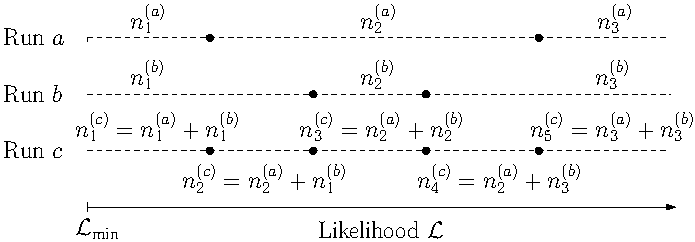
\includegraphics[width=0.8\textheight,angle=270]{figures/combine}
        \hfill
        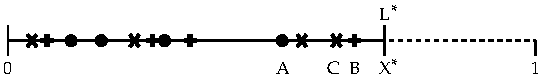
\includegraphics[width=0.8\textheight,angle=270]{figures/combine_0}
    \end{columns}
\end{frame}

\begin{frame}
    \frametitle{Birth $\mathcal{L}_*$ and death $\mathcal{L}$ contours}
    \begin{itemize}
        \item A nested sampling run is usually recorded in a database containing parameter values $\theta$, (log)likelihood $\mathcal{L}$, and optionally some expensive derived parameters $\phi$.
        \item The full nested sampling run can be losselessly reconstructed with an extra column.
        \item Namely the set of \textbf{birth contours}, i.e. the $\mathcal{L}_*$ at which each point was born at.
        \item With the lossless compression of columns $\mathcal{L}$ and $\mathcal{L}_*$, one can:
            \begin{itemize}
                \item Compute the dynamic number of live points,
                \item Reconstruct the nested sampling run history,
                \item Decompose an $n$-live point run into $n$ single live point runs.
            \end{itemize}
        \item Single live point runs form the indivisible unit of nested sampling.
        \item This post processing suite is encapsulated in the continuously integrated python packages of \texttt{anesthetic}~\arxiv{1905.04768} and \texttt{nestcheck}~\arxiv{1804.06406}.
    \end{itemize}

\end{frame}

\begin{frame}
    \frametitle{Parameter cross-checks}
    \begin{columns}
        \column{0.55\textwidth}
        \begin{itemize}
            \item ``Indivisible unit'' of nested sampling identified as the \emph{single live point run} (or \emph{thread}).
            \item When a nested sampling run is unwoven into its constituent threads, it can be recombined into smaller runs.
            \item Cross-checks such as bootstrap resampling can be applied to determine if these are consistent.
            \item This can be used to quantify the residual uncertainty in parameter estimation weights $w_i\approx L_i \Delta X_i$~\arxiv{1704.03459}.
                \begin{itemize}
                    \item in addition to Poisson uncertainty on $X_i$, there is also uncertainty associated with picking $\theta_i$ as representative of the entire $L_i$ contour~\arxiv{0801.3887}.
                \end{itemize}
        \end{itemize}
        \column{0.45\textwidth}
        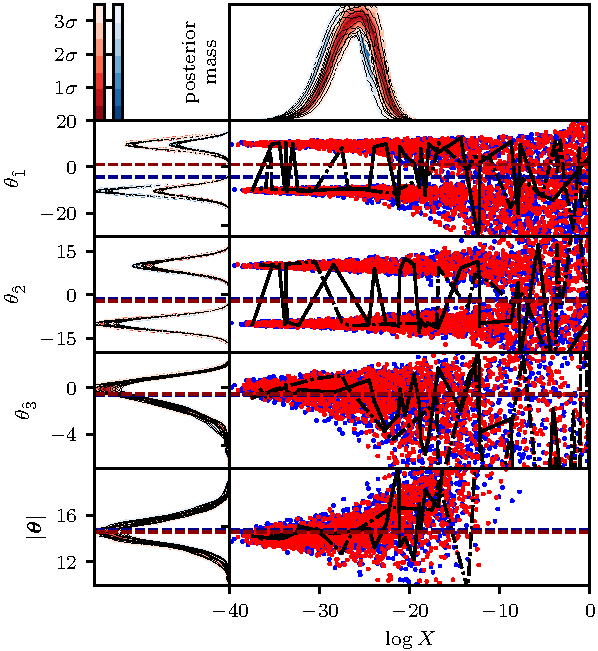
\includegraphics[width=\textwidth]{figures/nestcheck}
    \end{columns}
\end{frame}

\begin{frame}
    \frametitle{Insertion indices and order statistics}
    \begin{columns}
        \column{0.5\textwidth}
    \begin{itemize}
        \item At each iteration of nested sampling we generate a new live point and insert it into the list of live points sorted by loglikelihood.
        \item IF we have done things correctly, this should obey \emph{order statistics}.
        \item if it doesn't, our nested sampler is not drawing live points corectly;
        \item We demonstrate this with KS $p$-values~\arxiv{2006.03371}, to test reliability parameters.
        \item Should be extended to be more Bayesian.
        \item Needs extending to dynamic $n_\mathrm{live}$ case.
        \item This can be used at run-time to tune reliability parameters.
    \end{itemize}
        \column{0.5\textwidth}
        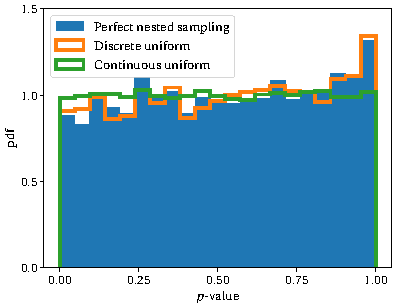
\includegraphics[width=\textwidth]{figures/indices}
    \end{columns}
\end{frame}

\begin{frame}
    \frametitle{Frontier: Insertion indices}

\begin{itemize}
    \item For the purposes of estimating volume in a statistical way, we discard the likelihood information, focussing on the ordering of the contours. 
    \item Traditional nested sampling uses the fact that
\[
    P(X_j|X_{j-1}, n_\mathrm{live}) = \frac{n_j}{X_{j-1}}\left( \frac{X_j}{X_{j-1}} \right)^{n_j-1} [0<X_j<X_{j-1}].
    \]
\item marginalised out dependency on everything other than $X_{j-1}$ \&  compressed into a vector encoding the number of live points at each iteration $n_i$. 
\item  \textbf{Frontier}: is ``Skilling compression'' $(\mathcal{L},\mathcal{L}_*)\to n$ lossless or lossy for the purposes of volume estimation?
\item The results presented in~\arxiv{2006.03371} are suggestive that it is losing some useful information, as insertion indexes do provide further information in the context of a cross check (and are in fact a lossless compression of the birth and death contours). 
\item One possibility is that the Skilling compression is lossless in the context of perfect nested sampling, but if a run is biased then you may be able to use insertion indexes to partially correct a biased run. 
\end{itemize}
\end{frame}

\begin{frame}
    \frametitle{Reversible nested sampling}
    \begin{itemize}
        \item One of the issues preventing nested sampling scaling to millions of dimensions is the need to compress from prior to posterior in all parameters.
            \begin{itemize}
                \item c.f. Skilling's argument that the Entropy/KL divergence is much greater than the width of the typical set/posterior bulk: $\mathcal{D}\sim d \gg \sqrt{d}$.
            \end{itemize}
        \item One could in principle reverse the direction of travel, and move outward from a peak.
        \item If one could guarantee that all peak looks gaussian close enough in (c.f. Laplace approximation), then one can estimate the final volume $X_N$, and reverse the usual argument.
        \item This could in principle be used to dramatically reduce the poisson error if one could estimate the volume in the final set of live points geometrically.
    \end{itemize}
\end{frame}

\begin{frame}
    \frametitle{AEONS: Approximating the end of nested sampling}
    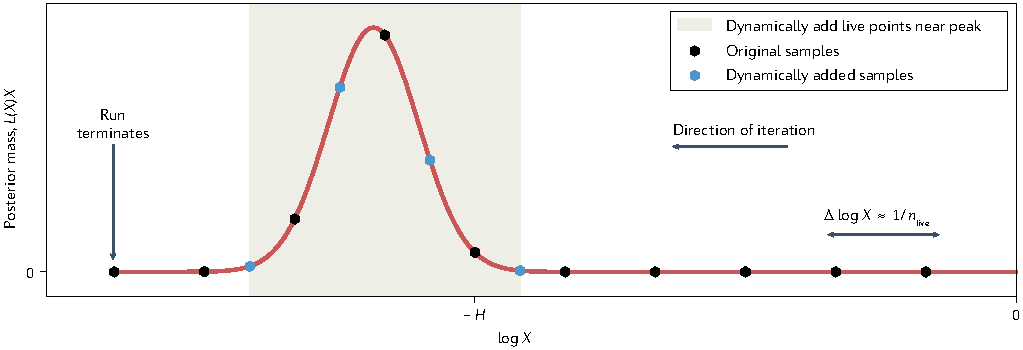
\includegraphics[width=\textwidth]{figures/run_prodecure}
    \vspace{-20pt}
    \begin{itemize}
        \item A seasoned user knows when nested sampling is approaching the end of an HPC run.
        \item As $\Delta\log \mathcal{Z}$ approaches unity, and there are only ``a few'' nested sampling iterations remaining before posterior is crossed.
        \item \textbf{Frontier:} Can we quantify this using Gaussian approximations to make a rough progress bar (with uncertainty quantification) -- summer student working on this.
    \end{itemize}
\end{frame}

\begin{frame}
    \frametitle{Importance nested sampling}
    \begin{columns}
    \column{0.5\textwidth}
    \begin{itemize}
        \item Importance sampling is the procedure:
            \begin{itemize}
                \item given a set of (weighted) samples $\{(w_i,\theta_i)\}$ drawn from posterior distribution $\mathcal{P}(\theta)$,
                \item If the likelihood $\mathcal{L}_0(\theta)=P(D_0|\theta)$ is updated with some additional data $D_1$, such that $\mathcal{L}_0 \to \mathcal{L}_0\times \mathcal{L}_1$~\arxiv{1902.04029},
                \item Can we re-weight $w_i$ without re-running a Markov Chain?
            \end{itemize}
        \item well-established for MCMC $w_i \to w_i \times L_1(\theta_i)$.
        \item For nested sampling, evidences are transformable $\mathcal{Z}_0\to \mathcal{Z}_0\times\langle L_1\rangle_{\mathcal{P}_0}$.
        \item Can we do better?
        \item \textbf{Frontier:} Is there a way to re-weight/thin a nested sampling run to recover the equivalent nested sampling run with a new likelihood?
    \end{itemize}
    \column{0.5\textwidth}
    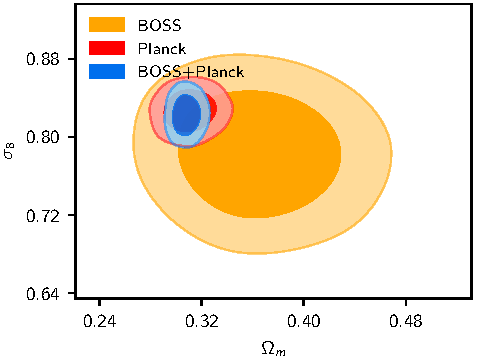
\includegraphics[width=\textwidth]{figures/importance}
    \end{columns}
\end{frame}

\begin{frame}
    \frametitle{Transdimensional nested sampling}
    \begin{columns}
        \column{0.5\textwidth}
        \begin{itemize}
            \item In some applications it is useful to consider parameter spaces where the number of active parameters vary, e.g.
                \begin{itemize}
                    \item Object detection~\arxiv{0809.3437},
                    \item Free-form reconstruction using \texttt{FlexKnots}~\arxiv{1908.00906}.
                \end{itemize}
            \item At the moment, reasonable performance can be achieved by letting $N$ be a parameter (up to $N_\mathrm{max}$) and then ignoring unused parameters~\arxiv{1506.09024}.
            \item Brendon Brewer~\arxiv{1411.3921} built some examples of RJMCMC diffusive nested sampling, but very problem specific.
            \item \textbf{Frontier:} Is there an ensemble-based methodology for transdimensional NS?
        \end{itemize}
        \column{0.5\textwidth}
        \includegraphics<1          >[width=\textwidth]{figures/recons1}
        \includegraphics<2|handout:0>[width=\textwidth]{figures/recons2}
    \end{columns}
\end{frame}


\begin{frame}
    \frametitle{Frontier: Multi-objective nested sampling}
    \begin{itemize}
        \item Nested sampling is useful as a pure optimiser, particularly for industrial applications where they lack likelihoods but have objective functions.
        \item It still provides a unique statistical interpretation for an arbitrary function $f(\theta)$ by providing a ``parameter compression'' $X_i\approx e^{i/n_\mathrm{live}} \leftrightarrow e^{\sum_j^i{1}/{n_j}}$ for each value of $f_i$.
        \item Also useful for providing a collection of solutions fairly distributed in parameter space once the desired optimum has been met.
        \item This collection of solutions is useful for rudimentary uncertainty quantification, but also for multi-objective optimisation.
        \item \textbf{Frontier}: Is there a more in-built multi-objective optimiser. Can nested sampling optimise two objective functions simultaneously up to a given compression?
    \end{itemize}
\end{frame}

\begin{frame}
    \frametitle{Likelihood values}
    \begin{columns}
        \column{0.5\textwidth}
    \begin{itemize}
        \item One of the virtues of nested sampling is that it only uses the ordering of likelihood values.
        \item \textbf{Frontier:} if one made a smoothness assumption, e.g. $\frac{d\log \mathcal{L}}{d\log X}\approx \mathrm{constant}$, is is possible to do better?
        \item This could dramatically reduce the poisson error, runtime and efficiency of NS.
    \end{itemize}
    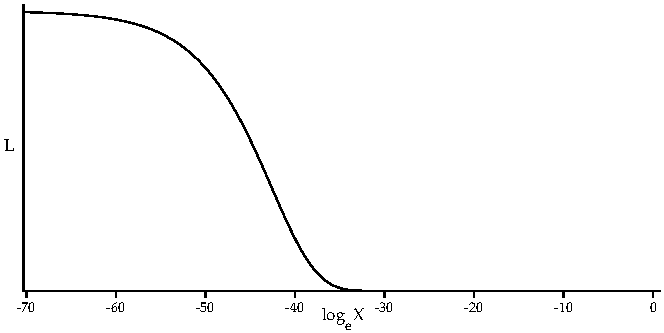
\includegraphics[width=\textwidth]{figures/values1}
        \column{0.5\textwidth}
    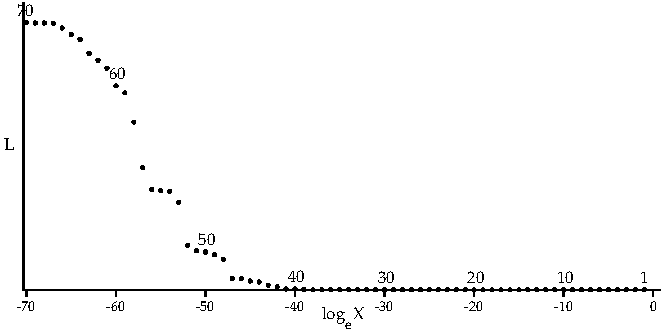
\includegraphics[width=\textwidth]{figures/values}
    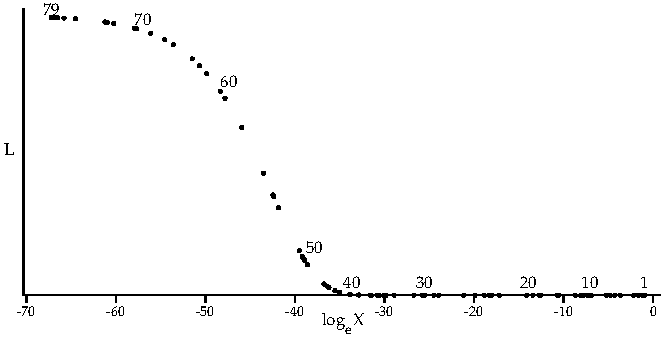
\includegraphics[width=\textwidth]{figures/values2}
    \end{columns}
\end{frame}


\begin{frame}
    \frametitle{Nested Sampling with Likelihood Free Inference}
    \begin{columns}
        \column{0.5\textwidth}
        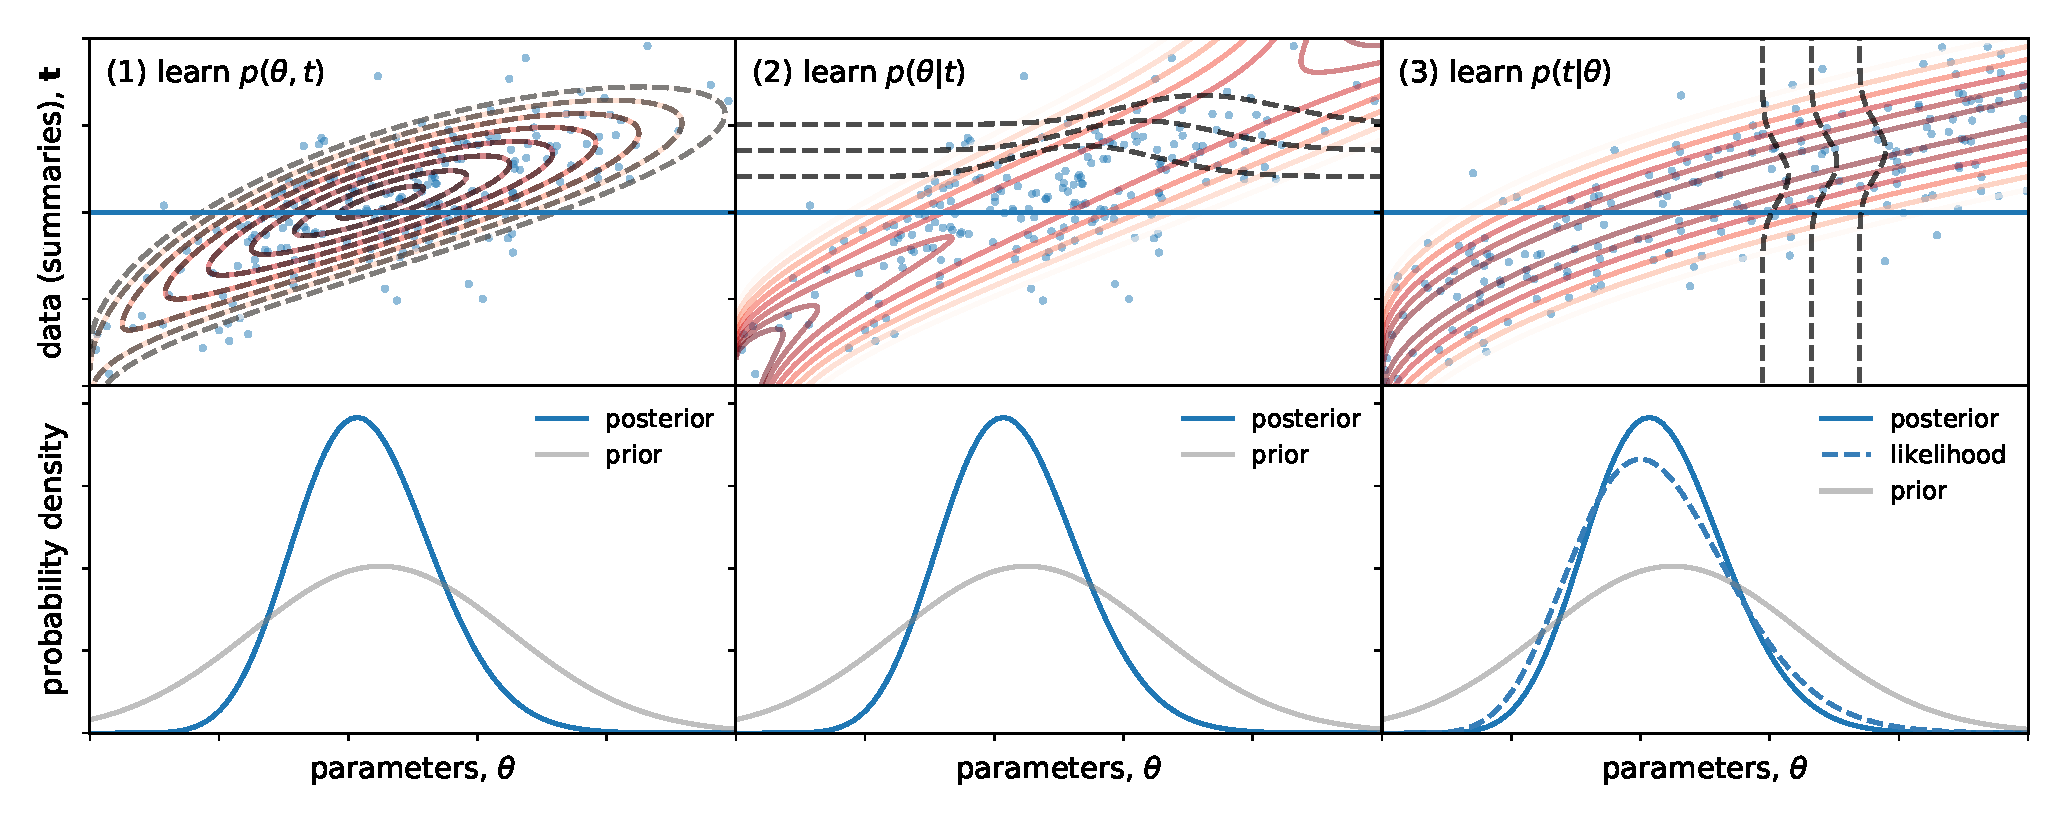
\includegraphics[width=\textwidth]{figures/three_ways_II.pdf}

        \hfill Alsing \textit{et al.}~\arxiv{1903.00007}
    \begin{itemize}
        \item In density estimation likelihood free inference, the output is to learn one/all of:
            \begin{description}
                \item[Likelihood] $P(D|\theta)$,
                \item[Posterior] $P(\theta|D)$,
                \item[Joint] $P(D,\theta)$.
            \end{description}
        \item In the first instance, nested sampling can be used to scan these learnt functions.
    \end{itemize}
        \column{0.5\textwidth}
    \begin{itemize}
        \item Data are compressed, so joint space $(D,\theta)$ is navigable by off-the-shelf codes. 
            \begin{itemize}
                \item Sanity checking the solution,
                \item Computing evidences/Kullback Liebler divergences from likelihoods.
            \end{itemize}
        \item Its self-tuning capacity and ability to handle multi-modal distributions can be very useful for diagnosing incompletely learnt functions.
        \item Emulated likelihoods (e.g. normalising flows) are generally fast, so can deploy more likelihood hungry techniques like NS.
        \item In principle can use it to train emulators by marginalisation rather than maximisation.
    \end{itemize}
    \end{columns}
\end{frame}

\begin{frame}
    \frametitle{Nested Sampling for Approximate Bayesian Computation/SBI}
    \begin{columns}
        \column{0.5\textwidth}
        \begin{itemize}
            \item Assume one has a generative model capable of turning parameters into mock data $D(\theta)$.
            \item Given infinite computing power, ABC works by selecting $\{\theta : D(\theta)=D_\mathrm{observed}\}$.
            \item These are samples from the posterior, without using a likelihood.
            \item In practice $D=D_\mathrm{obs}$ becomes $D\approx D_\mathrm{obs}$.
            \item i.e. $|D-D_\mathrm{obs}|<\varepsilon$, or more generally $\boxed{\rho(D,D_\mathrm{obs})<\varepsilon}$, where $\rho$ is some suitably chosen objective function.
            \item Main challenges are 
                \begin{enumerate}
                    \item Choice of $\rho$/summary stats,
                    \item Choice of $\varepsilon$ schedule,
                    \item Rejection sampling.
                \end{enumerate}
        \end{itemize}
        \column{0.5\textwidth}
        \begin{itemize}
            \item Nested sampling fits this well: In principle, can just change the usual hard likelihood constraints $\{\theta\sim\pi : \mathcal{L}(\theta)>\mathcal{L}_*\}$ to
                \[\{\theta~\sim\pi : \rho(D(\theta),D_\mathrm{obs})<\varepsilon\}\]
            (Brewer \& Foreman-Mackey~\arxiv{1606.03757})
            \item Ongoing work with Andrew Fowlie \& Sebastian Hoof
                \begin{itemize}
                    \item How to deal with nondeterminism,
                    \item How to interpret $\rho$ as a ``likelihood'',
                    \item How to interpret the evidence $\mathcal{Z}$.
                \end{itemize}
        \end{itemize}
    \end{columns}
\end{frame}

%\begin{frame}
%    \frametitle{Nested sampling for truncated methods}
%
%    \begin{columns}
%        \column{0.55\textwidth}
%        \begin{itemize}
%            \item Will hear more on this tomorrow from Christoph
%            \item Many Likelihood implicit approaches at the moment have some element of sampling direct from the prior
%            \item Inefficient if number of parameters $>\mathcal{O}(\text{a few})$
%            \item Can get round this by truncating to region:
%                \[ \Gamma\{ \theta\in \mathrm{supp} p(\theta) \:|\: p(\theta|x_0)>\bar\varepsilon\} \]
%            \item At the moment regions defined by nested boxes
%            \item \textbf{Frontier:} This seems ripe for replacement by NS -- PhD student currently working on this (Kilian Scheutwinkel)
%        \end{itemize}
%        \column{0.45\textwidth}
%        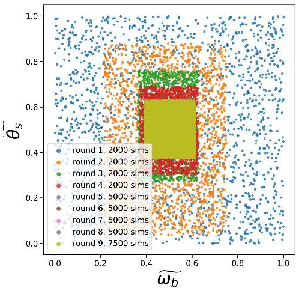
\includegraphics[width=\textwidth]{figures/tmnre}
%
%        \hfill Cole \textit{et al.}~\arxiv{2111.08030}
%    \end{columns}
%    
%\end{frame}



\begin{frame}
    \frametitle{Conclusions}
    \begin{itemize}
        \item Nested sampling is a truly unique tool -- the only general-purpose probabalistic integrator
    \end{itemize}
    \vspace{-12pt}
    \begin{columns}[t]
        \small
        \hspace{10pt}
        \column{0.33\textwidth}
        \begin{itemize}
            \itemsep0em
            \item Rejection and chain-based nested sampling,
            \item Dynamic nested sampling,
            \item Unweaving runs,
            \item Birth and death contours,
            \item Importance nested sampling,
        \end{itemize}
        \column{0.33\textwidth}
        \begin{itemize}
            \itemsep0em
            \item Cross checks,
            \item Insertion indices and order statistics,
            \item Reversible nested sampling,
            \item AEONS,
        \end{itemize}
        \column{0.33\textwidth}
        \begin{itemize}
            \itemsep0em
            \item Transdimensional nested sampling,
            \item Multiobjective nested sampling,
            \item Using likelihood values,
            \item Likelihood free inference.
        \end{itemize}
    \end{columns}
    \begin{block}{Watch out for:}
        \begin{description}
            \item[Johannes Buchner (next)] Analysing chain based samplers.
            \item[Aleksandr Petrosyan (before coffee)] Accelerating nested sampling.
            \item[Livia Partay (after coffee)] Nested sampling in materials science.
            \item[Lune Maillard (after Livia)] Nested sampling and free energy surfaces.
            \item[Harry Bevins (Friday before lunch)] Nested sampling and normalising flows.
        \end{description}
    \end{block}
\end{frame}

\appendix


\begin{frame}
    \frametitle{How does Nested Sampling compare to other approaches?}
    \begin{columns}
        \column{0.7\textwidth}
        \begin{itemize}
            \item In all cases:
                \begin{itemize}
                    \item[$+$] NS can handle multimodal functions
                    \item[$+$] NS computes evidences, partition functions and integrals
                    \item[$+$] NS is self-tuning/black-box
                \end{itemize}
        \end{itemize}
        \column{0.3\textwidth}
        Modern Nested Sampling algorithms can do this in $\sim\mathcal{O}(100s)$ dimensions
    \end{columns}
    \begin{columns}[t]
        \column{0.33\textwidth}
        \begin{block}{Optimisation}
            \begin{itemize}
                \item Gradient descent
                    \begin{itemize}
                        \item[$+$] NS does not require gradients
                    \end{itemize}
                \item Genetic algorithms
                    \begin{itemize}
                        \item[$+$] NS discarded points have statistical meaning
                    \end{itemize}
            \end{itemize}
        \end{block}
        \column{0.33\textwidth}
        \begin{block}{Sampling}
            \begin{itemize}
                \item Metropolis-Hastings?
                    \begin{itemize}
                        \item[$-$] Very little beats a well-tuned, customised MH
                        \item[$+$] NS is self tuning
                    \end{itemize}
                \item Hamiltonian Monte Carlo?
                    \begin{itemize}
                        \item[$-$] In millions of dimensions, HMC is king
                        \item[$+$] NS does not require gradients
                    \end{itemize}
            \end{itemize}
        \end{block}
        \column{0.33\textwidth}
        \begin{block}{Integration}
            \begin{itemize}
                \item Thermodynamic integration
                    \begin{itemize}
                        \item[$+$] protective against phase trasitions
                        \item[$+$] No annealing schedule tuning 
                    \end{itemize}
                \item Sequential Monte Carlo
                    \begin{itemize}
                        \item[$-$] Some people (SMC experts) classify NS as a kind of SMC
                        \item[$+$] NS is athermal
                    \end{itemize}
            \end{itemize}
        \end{block}
    \end{columns}
\end{frame}

\begin{frame}
    \frametitle{Nested Sampling: a user's guide}
    \begin{enumerate}
        \item Nested sampling is a likelihood scanner, rather than posterior explorer.
            \begin{itemize}
                \item This means typically most of its time is spent on burn-in rather than posterior sampling.
                \item Changing the stopping criterion from $10^{-3}$ to $0.5$ does little to speed up the run, but can make results very unreliable.
            \end{itemize}
        \item The number of live points $n_\mathrm{live}$ is a resolution parameter.
            \begin{itemize}
                \item Run time is linear in $n_\mathrm{live}$, posterior and evidence accuracy goes as $\frac{1}{\sqrt{n_\mathrm{live}}}$.
                \item Set low for exploratory runs $\sim\mathcal{O}(10)$ and increased to $\sim\mathcal{O}(1000)$ for production standard.
            \end{itemize}
        \item Most algorithms come with additional reliability parameter(s).
            \begin{itemize}
                \item e.g. \texttt{MultiNest}: $\texttt{eff}$, \texttt{PolyChord}: $n_\mathrm{repeats}$.
                \item These are parameters which have no gain if set too conservatively, but increase the reliability.
                \item Check that results do not degrade if you reduce them from defaults, otherwise increase.
            \end{itemize}
    \end{enumerate}
\end{frame}




\end{document}
